\section{Specifying a Graph of Lists, Maps, and Registers}\label{sec:datatypes}

We now make the OpSets approach concrete by defining example semantics for commonly-used data structures: maps (which associate values with user-specified keys) and lists (linear sequences of values).
The map datatype can also represent a set (by using keys as members of the set, and ignoring values).
The list datatype can also represent text (by mapping each character to a list element).
In both lists and maps the values may be primitives (such as numbers or strings), or references to other map or list objects.
Using these references we can construct arbitrary object graphs, including cycles of object references, like in object-oriented programming languages.
In Section~\ref{sec:tree} we will show how to restrict this object graph so that it conforms to a tree structure.

We treat each key of a map, and each element of a list, as a multi-value register.
That is, if there are several concurrent assignments to the same map key or list element, our datatype preserves all concurrently written values.
Thus, reading a map key or list element may return multiple values, which may be merged explicitly by the user.
Assigning a new value to a map key or list elements overwrites all causally preceding values.
Different register behaviour, such as last-writer-wins (arbitrarily picking one of the concurrently written values as winner), can easily be defined, as we show later.

\subsection{Generating Operations}\label{sec:datatypes-gen}

An OpSet for these datatypes may contain six types of operation:
\begin{description}
    \item[$(\mathit{id},\, \mathsf{MakeMap})$] creates a new, empty map object.
        $\mathit{id}$ may henceforth be used to identify this object.
    \item[$(\mathit{id},\, \mathsf{MakeList})$] creates a new, empty list object.
        $\mathit{id}$ may henceforth be used to identify this object.
    \item[$(\mathit{id},\, \mathsf{MakeVal}(\mathit{val}))$] associates the ID $\mathit{id}$ with the primitive value $\mathit{val}$ (e.g.\ a number, string, or boolean).
        This operation is used to ``wrap'' any primitive value, allowing $\mathsf{Assign}$ operations (see below) to always use IDs as values, regardless of whether the value is a primitive value, or a reference to a map or list object.
    \item[$(\mathit{id},\, \mathsf{InsertAfter}(\mathit{ref}))$] creates a new list element with ID $\mathit{id}$, and inserts it into a list.
        If $\mathit{ref}$ is the ID of a prior $\mathsf{MakeList}$ operation, then the new element is inserted at the head of that list.
        Otherwise $\mathit{ref}$ must be the ID of an existing list element (i.e.\ a prior $\mathsf{InsertAfter}$ operation), in which case the new list element is inserted immediately after the referenced list element.
        Note that the $\mathsf{InsertAfter}$ operation does not associate a value with the new list element; that is done by a subsequent $\mathsf{Assign}$ operation.
    \item[$(\mathit{id},\, \mathsf{Assign}(\mathit{obj}, \mathit{key}, \mathit{val}, \mathit{prev}))$] assigns a new value to a key within a map (if $\mathit{obj}$ is the ID of a prior $\mathsf{MakeMap}$ operation), or to a list element (if $\mathit{obj}$ is the ID of a prior $\mathsf{MakeList}$ operation).
        In the case of map assignment, $\mathit{key}$ is the user-specified key to be updated, which may be any primitive value such as a string or integer.
        In the case of a list, $\mathit{key}$ is the ID of the list element to be updated (i.e.\ the ID of a prior $\mathsf{InsertAfter}$ operation).
        $\mathit{val}$ is the ID of the value being assigned, which may identify a $\mathsf{MakeMap}$, $\mathsf{MakeList}$, or $\mathsf{MakeVal}$ operation.
        $\mathit{prev}$ is the set of IDs of prior $\mathsf{Assign}$ operations to the same key in the same object, which are overwritten by the present operation.
    \item[$(\mathit{id},\, \mathsf{Remove}(\mathit{obj}, \mathit{key}, \mathit{prev}))$] removes a key-value pair from a map, or an element from a list.
        As with $\mathsf{Assign}$, $\mathit{obj}$ is the ID of the prior $\mathsf{MakeMap}$ or $\mathsf{MakeList}$ operation that created the object being updated, and $\mathit{key}$ identifies the key or list element being removed.
        $\mathit{prev}$ is the set of IDs of prior $\mathsf{Assign}$ operations to the same key in the same object, which are removed by the present operation.
\end{description}

\floatname{algorithm}{Listing}
\begin{algorithm}[t]
\caption{Generating new operations for modifying maps and lists.}\label{fig:pseudocode}
\noindent
\renewcommand\algorithmicindent{10pt}
\begin{minipage}[t]{0.5\textwidth}
\begin{algorithmic}
    \Function{setMapKey}{$O, \mathit{map}, \mathit{key}, \mathit{val}$}
    \State $(E,\, L) = \llbracket O \rrbracket$
    \State $(\mathit{id}_1, \mathit{op}_1) = \Call{valueID}{O, \mathit{val}}$
    \State $O' = (\textbf{if } \mathit{op}_1 = \bot \textbf{ then } O \textbf{ else } 
        O \;\cup\; \big\{ (\mathit{id}_1, \mathit{op}_1) \big\})$
    \State $\mathit{id}_2 = \mathrm{newID}(O')$
    \State $\mathit{prev} = \{ \mathit{id} \mid \exists\,v.\; (\mathit{id}, \mathit{map}, \mathit{key}, v) \in E \}$
    \State \Return $O' \;\cup\; \big\{ (\mathit{id}_2,\, \mathsf{Assign}(\mathit{map}, \mathit{key}, \mathit{id}_1, \mathit{prev})) \big\}$
    \EndFunction\Statex

    \Function{removeMapKey}{$O, \mathit{map}, \mathit{key}$}
    \State $(E,\, L) = \llbracket O \rrbracket$
    \State $\mathit{id}_1 = \mathrm{newID}(O)$
    \State $\mathit{prev} = \{ \mathit{id} \mid \exists\,v.\; (\mathit{id}, \mathit{map}, \mathit{key}, v) \in E \}$
    \State \Return $O \;\cup\; \big\{ (\mathit{id}_1,\, \mathsf{Remove}(\mathit{map}, \mathit{key}, \mathit{prev})) \big\}$
    \EndFunction\Statex

    \Function{valueID}{$O, \mathit{val}$}
    \If{$\mathit{val}$ is a primitive type}
    \State \Return $(\mathrm{newID}(O),\, \mathsf{MakeVal}(\mathit{val}))$
    \ElsIf{$\mathit{val} = \texttt{[]}$ (empty list literal)}
    \State \Return $(\mathrm{newID}(O),\, \mathsf{MakeList})$
    \ElsIf{$\mathit{val} = \texttt{{\char '173}{\char '175}}$ (empty map literal)}
    \State \Return $(\mathrm{newID}(O),\, \mathsf{MakeMap})$
    \Else ~($\mathit{val}$ is an existing object)
    \State \Return $(\mathrm{objID}(\mathit{val}),\, \bot)$
    \EndIf
    \EndFunction
\end{algorithmic}
\end{minipage}%
\begin{minipage}[t]{0.5\textwidth}
\begin{algorithmic}
    \Function{setListIndex}{$O, \mathit{list}, \mathit{index}, \mathit{val}$}
    \State $(E,\, L) = \llbracket O \rrbracket$
    \State $(\mathit{id}_1, \mathit{op}_1) = \Call{valueID}{O, \mathit{val}}$
    \State $O' = (\textbf{if } \mathit{op}_1 = \bot \textbf{ then } O \textbf{ else } 
        O \;\cup\; \big\{ (\mathit{id}_1, \mathit{op}_1) \big\})$
    \State $\mathit{id}_2 = \mathrm{newID}(O')$
    \State $\mathit{key} = \mathrm{idxKey}_{E,\, L}(\mathit{list}, \mathit{list}, \mathit{index})$
    \State $\mathit{prev} = \{ \mathit{id} \mid \exists\,v.\; (\mathit{id}, \mathit{list}, \mathit{key}, v) \in E \}$
    \State \Return $O' \;\cup\; \big\{ (\mathit{id}_2,\, \mathsf{Assign}(\mathit{list}, \mathit{key}, \mathit{id}_1, \mathit{prev})) \big\}$
    \EndFunction\Statex

    \Function{insertListIndex}{$O, \mathit{list}, \mathit{index}, \mathit{val}$}
    \State $(E,\, L) = \llbracket O \rrbracket$
    \State $(\mathit{id}_1, \mathit{op}_1) = \Call{valueID}{O, \mathit{val}}$
    \State $O' = (\textbf{if } \mathit{op}_1 = \bot \textbf{ then } O \textbf{ else } 
        O \;\cup\; \big\{ (\mathit{id}_1, \mathit{op}_1) \big\})$
    \State $\mathit{id}_2 = \mathrm{newID}(O')$
    \State $\mathit{ref} = (\textbf{if } \mathit{index}=0 \textbf{ then } \mathit{list}$
    \State $\hphantom{\mathit{ref} = (}\textbf{else } \mathrm{idxKey}_{E,\, L}(\mathit{list}, \mathit{list}, \mathit{index} - 1))$
    \State $O'' = O' \;\cup\; \big\{ (\mathit{id}_2,\, \mathsf{InsertAfter}(\mathit{ref})) \big\}$
    \State $\mathit{id}_3 = \mathrm{newID}(O'')$
    \State \Return $O'' \;\cup\; \big\{ (\mathit{id}_3,\, \mathsf{Assign}(\mathit{list}, \mathit{id}_2, \mathit{id}_1, \emptyset)) \big\}$
    \EndFunction\Statex

    \Function{removeListIndex}{$O, \mathit{list}, \mathit{index}$}
    \State $(E,\, L) = \llbracket O \rrbracket$
    \State $\mathit{id}_1 = \mathrm{newID}(O)$
    \State $\mathit{key} = \mathrm{idxKey}_{E,\, L}(\mathit{list}, \mathit{list}, \mathit{index})$
    \State $\mathit{prev} = \{ \mathit{id} \mid \exists\,v.\; (\mathit{id}, \mathit{list}, \mathit{key}, v) \in E \}$
    \State \Return $O \;\cup\; \big\{ (\mathit{id}_1,\, \mathsf{Remove}(\mathit{list}, \mathit{key}, \mathit{prev})) \big\}$
    \EndFunction
\end{algorithmic}
\end{minipage}
\end{algorithm}

\noindent
Listing~\ref{fig:pseudocode} gives pseudocode for functions that generate these operations.
The first parameter $O$ of each function is the OpSet that defines the current state of the node, and the functions return an updated OpSet containing new operations.
The interpretation $\llbracket O \rrbracket$ returns a pair $(E,\, L)$ as defined in Section~\ref{sec:datatypes-interp}.
The function $\mathrm{newID}(O)$ returns a unique ID (e.g.\ a Lamport timestamp) that is greater than any existing ID in the OpSet $O$.

The function \textsc{setMapKey} can be called by a user to update a map object with ID $\mathit{map}$, setting a key $\mathit{key}$ to a value $\mathit{val}$.
If $\mathit{val}$ references an existing object, $\mathit{id}_1$ is set to the ID of that existing object; otherwise, the function \textsc{valueID} generates a new $\mathsf{Make}\cdots$ operation for the value, and the new operation is added to $O'$.
A new ID $\mathit{id}_2$ is generated for the $\mathsf{Assign}$ operation, in which the key $\mathit{key}$ is set to $\mathit{id}_1$ (which identifies the value $\mathit{val}$).
Finally, the function returns the OpSet with the $\mathsf{Assign}$ operation included.
The other function definitions follow a similar pattern.

The list manipulation functions \textsc{setListIndex}, \textsc{insertListIndex} and \textsc{removeListIndex} take a numeric index as argument to identify the position in the list being edited.
The numeric index is translated into the ID of a list element using the function $\mathrm{idxKey}_{E,\, L}()$, which is defined in Section~\ref{sec:datatypes-interp}.

\subsection{Interpreting Operations}\label{sec:datatypes-interp}

We use the sequential OpSet interpretation given in Section~\ref{sec:op-serial}.
To encode the current state of map and list data structures we use a pair of relations $(E,\, L)$:
\begin{description}
    \item[The element relation $E \subseteq (\mathrm{ID} \times \mathrm{ID} \times (\mathrm{ID} \cup \mathrm{Key}) \times \mathrm{ID})$]
        is a set of 4-tuples containing the values currently assigned to map keys and list elements.
        If $(\mathit{id}, \mathit{obj}, \mathit{key}, \mathit{val}) \in E$, then an $\mathsf{Assign}$ operation with ID $\mathit{id}$ updated the object with ID $\mathit{obj}$, assigning the value with ID $\mathit{val}$ to the map key or list element $\mathit{key}$.
        If $\mathit{obj}$ references a list object, $\mathit{key}$ is the ID of an element in the list relation $L$ (see below).
        If $\mathit{obj}$ references a map object, any primitive value such as string or integer may be used as $\mathit{key}$.
    \item[The list relation $L \subseteq (\mathrm{ID} \times \mathrm{ID})$] is a set of pairs that indicates the order of list elements.
        If $(\mathit{prev}, \mathit{next}) \in L$, that means the list element with ID $\mathit{prev}$ is immediately followed by the list element with ID $\mathit{next}$.
        We use $(\mathit{last}, \bot) \in L$ to indicate that list element $\mathit{last}$ has no successor.
        To indicate that $\mathit{head}$ is the first element in the list $\mathit{obj}$ (i.e.\ $\mathit{obj}$ is the ID of the $\mathsf{MakeList}$ operation that created the list) we have $(\mathit{obj}, \mathit{head}) \in L$.
\end{description}
Initially, both relations are empty; that is, we have $\llbracket\emptyset\rrbracket = \mathit{InitialState} = (\emptyset,\, \emptyset)$.
We can then define the interpretation of the six operation types as follows:
\begin{align*}
    \mathit{interp}\big[(E,\, L),\, (\mathit{id},\, \mathsf{Assign}(\mathit{obj}, k, v, \mathit{prev})) \big] &\;=\; \Big(
    \big\{ (\mathit{id}', \mathit{obj}', k', v') \in E \mid
    \mathit{id}' \notin \mathit{prev} \big\} \;\cup\;
    \big\{ (\mathit{id}, \mathit{obj}, k, v) \big\},\; L \Big) \\[5pt]
    %%%%%%%%%%
    \mathit{interp}\big[(E,\, L),\, (\mathit{id},\, \mathsf{Remove}(\mathit{obj}, k, \mathit{prev})) \big] &\;=\; \Big(
    \big\{ (\mathit{id}', \mathit{obj}', k', v') \in E \mid
    \mathit{id}' \notin \mathit{prev} \big\},\; L \Big) \\[5pt]
    %%%%%%%%%%
    \mathit{interp}\big[(E,\, L),\, (\mathit{id},\, \mathsf{InsertAfter}(r)) \big] &\;=\; \left\{
        \arraycolsep=0pt \def\arraystretch{1.2}
        \begin{array}{ll}
            (E,\, L) & \text{if } \nexists\,n.\; (r,\, n) \in L\\[3pt]
            \Big(E,\; \big\{ (p,n) \;&\in L \mid p \neq r \big\} \;\cup\;
            \big\{ (r, \mathit{id}) \big\} \;\cup\;
            \big\{ (\mathit{id}, n) \mid (r, n) \in L \big\} \Big)\\
            & \text{if } \exists\,n.\; (r,\,n) \in L
        \end{array} \right. \\[5pt]
    %%%%%%%%%%
    \mathit{interp}\big[(E,\, L),\, (\mathit{id},\, \mathsf{MakeList}) \big] &\;=\; \Big(
    E,\; L \;\cup\; \big\{(\mathit{id},\, \bot)\big\}\Big) \\[5pt]
    %%%%%%%%%%
    \mathit{interp}\big[(E,\, L),\, (\mathit{id},\, \mathsf{MakeMap}) \big] &\;=\; \mathit{interp}\big[(E,\, L),\, (\mathit{id},\, \mathsf{MakeVal}(\mathit{val})) \big] \;=\; (E,\; L)
\end{align*}

The interpretation of $\mathsf{Assign}$ and $\mathsf{Remove}$ updates only $E$ and leaves $L$ unchanged; conversely, the interpretation of $\mathsf{InsertAfter}$ and $\mathsf{MakeList}$ updates only $L$.
Both the $\mathsf{Assign}$ and $\mathsf{Remove}$ interpretations remove any tuples from causally prior assignments (those whose IDs appear in $\mathit{prev}$), but leave any tuples from concurrent assignments unchanged.
This is the behaviour of a multi-value register; if a last-writer-wins register is required, the condition $\mathit{id}' \notin \mathit{prev}$ can be changed to $\mathit{obj}' \neq \mathit{obj} \;\vee\; k' \neq k$, which removes any existing tuples with the same object ID and key.

The interpretation of $\mathsf{InsertAfter}$ resembles the insertion into a linked list, as illustrated in Figure~\ref{fig:list-insert}.
For example, to interpret $(\mathit{id},\, \mathsf{InsertAfter}(r))$, if we have $(r, n) \in L$, we remove the pair $(r, n)$ from L, and add the pairs $(r, \mathit{id})$ and $(\mathit{id}, n)$ to $L$.
Thus, the new list element $\mathit{id}$ is inserted between $r$ and $n$.

\begin{figure}
\centering
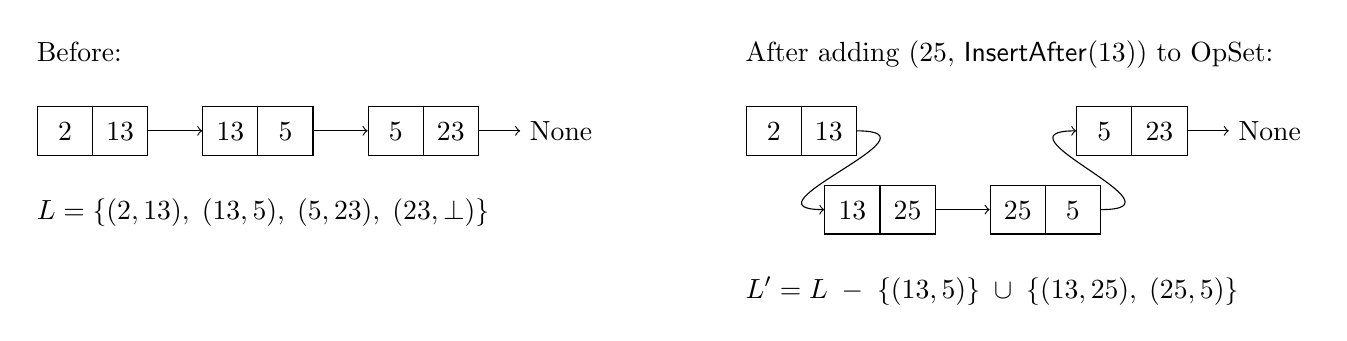
\begin{tikzpicture}
  \tikzstyle{every node}=[anchor=base,minimum width=7mm,text height=9pt,text depth=2pt]
  \node [anchor=west] at (-9,2) {Before:};
  \node [anchor=west] at (-9,0) {$L = \{ (2, 13),\; (13, 5),\; (5, 23),\; (23, \bot) \}$};
  \node [anchor=west] at (0,2) {After adding $(25,\, \mathsf{InsertAfter}(13))$ to OpSet:};
  \node [anchor=west] at (0,-1) {$L' = L \;-\; \{(13, 5)\} \;\cup\; \{(13, 25),\; (25, 5)\}$};
    \matrix [column sep={7mm,between origins},nodes=draw,matrix anchor=west] at (-9,1) {
    \node (l1a) {2};  & \node (l1b) {13}; &&
    \node (l2a) {13}; & \node (l2b) {5};  &&
    \node (l3a) {5};  & \node (l3b) {23}; &&
    \node (l4a) [draw=none] {None}; \\
  };
  \draw [->] (l1b) -- (l2a);
  \draw [->] (l2b) -- (l3a);
  \draw [->] (l3b) -- (l4a);
  \matrix [column sep={7mm,between origins},nodes=draw,matrix anchor=west] at (1,0) {
    \node (n1) {13}; & \node (n2) {25}; &&
    \node (n3) {25}; & \node (n4) {5}; \\
  };
  \matrix [column sep={7mm,between origins},nodes=draw,matrix anchor=west] at (0,1) {
    \node (r1a) {2};  & \node (r1b) {13}; &&&&&
    \node (r3a) {5};  & \node (r3b) {23}; &&
    \node (r4a) [draw=none] {None}; \\
  };
  \draw [->] (r1b.east) .. controls (2.7,1) and (0,0) .. (n1.west);
  \draw [->] (n2) -- (n3);
  \draw [->] (n4.east) .. controls (5.8,0) and (3.2,1) .. (r3a.west);
  \draw [->] (r3b) -- (r4a);
\end{tikzpicture}
\caption{Illustration of the interpretation of an $\mathsf{InsertAfter}$ operation.}\label{fig:list-insert}
\end{figure}

Note that $L$ never shrinks, it only ever grows through interpreting $\mathsf{InsertAfter}$ operations.
When a list element is removed by the function \textsc{removeListIndex} of Listing~\ref{fig:pseudocode}, the effect is that all values are removed from the list element in the element relation $E$, but the list element remains in $L$ as a \emph{tombstone}, so that any concurrent $\mathsf{InsertAfter}$ operations can still locate the referenced list position.

Thus, from a user's point of view a list element only exists if it has at least one associated value in the $E$ relation; any list elements without an associated value should be ignored.
On this basis we can now define the $\mathrm{idxKey}()$ function that is used in Listing~\ref{fig:pseudocode} to translate a list index into a list element ID:
\[ \mathrm{idxKey}_{E,\, L}(\mathit{obj}, \mathit{key}, i) \;=\; \left\{
   \arraycolsep=2pt \def\arraystretch{1.3}
   \begin{array}{llllll}
       \mathrm{idxKey}_{E,\, L}(\mathit{obj}, n, i-1) &
       \quad\text{if }\; i > 0 & \wedge & (\mathit{key}, n) \in L & \wedge &
       \exists\,\mathit{id}, \mathit{val}.\; (\mathit{id}, \mathit{obj}, \mathit{key}, \mathit{val}) \in E \\
       \mathrm{idxKey}_{E,\, L}(\mathit{obj}, n, i) &
       \quad\text{if }\; && (\mathit{key}, n) \in L & \wedge &
       \nexists\,\mathit{id}, \mathit{val}.\; (\mathit{id}, \mathit{obj}, \mathit{key}, \mathit{val}) \in E \\
       \mathit{key} &
       \quad\text{if }\; i = 0 & \wedge &&&
       \exists\,\mathit{id}, \mathit{val}.\; (\mathit{id}, \mathit{obj}, \mathit{key}, \mathit{val}) \in E \\
   \end{array} \right. \]
$\mathit{key}$ is initially the ID of the $\mathsf{MakeList}$ operation that created the list.
The function recursively moves along the linked list structure in $L$, decrementing the index for every list element that has an associated value, and not counting any list elements without associated value (which are treated as deleted).
Eventually, it returns the ID of the list element with the desired index.
